% -*- TeX:de -*-
\NeedsTeXFormat{LaTeX2e}
\documentclass[12pt,a4paper]{article}
\usepackage[english]{babel} % german text
\usepackage[DIV12]{typearea} % size of printable area
\usepackage[T1]{fontenc} % font encoding
%\usepackage[latin1]{inputenc} % most likely on Windows
\usepackage[utf8]{inputenc} % probably on Linux
\usepackage{multicol}
% PLOTTING
\usepackage{pgfplots}
\usepackage{pgfplotstable}
\usepackage{url}
\usepackage{graphicx} % to include images
\usepackage{tikz}
\usepackage{subfigure} % for creating subfigures
\usepackage{amsmath} % a bunch of symbols
\usepackage{amssymb} % even more symbols
\usepackage{booktabs} % pretty tables
\usepackage{makecell} % multi row table heading
% a floating environment for circuits
\usepackage{float}
\usepackage{caption}
\usepackage{hyperref}
\usepackage{eurosym}

% Title Page command
\newcommand{\HRule}{\rule{\linewidth}{0.5mm}}

%\newfloat{circuit}{tbph}{circuits}
%\floatname{circuit}{Schaltplan}
% a floating environment for diagrams
%\newfloat{diagram}{tbph}{diagrams}
%\floatname{diagram}{Diagramm}
\pgfplotsset{compat=1.8}
\selectlanguage{english} % use german
\begin{document}
%%%%%%% DECKBLATT %%%%%%%
\begin{titlepage}
\begin{center}

% Upper part of the page. The '~' is needed because \\
% only works if a paragraph has started.

\includegraphics[scale=0.75]{./unilogo}~\\[2cm]

\textsc{\LARGE University of Vienna }\\[0.5cm]
\textsc{\LARGE Faculty of Physics}\\[1.5cm]
\textsc{\Large Quantum optics practical course}\\[0.5cm]

% Title
\HRule \\[0.4cm]
{ \huge \bfseries Radiaton Pressure}\\[0.4cm]

\HRule \\[1.5cm]

% Author and supervisor
\begin{minipage}{0.4\textwidth}
\begin{flushleft} \large
\emph{Author:}\\
Johannes \textsc{Kurz}\\
\emph{Group:}\\
\textsc{Braun, Donabaum, Kurz}\\
\end{flushleft}
\end{minipage}
\begin{minipage}{0.4\textwidth}
\begin{flushright} \large
\emph{Supervisor:} \\
Witlef \textsc{Wieczorek}
\end{flushright}
\end{minipage}

\vfill

% Bottom of the page
{\large 31.10.2014}

\end{center}
\end{titlepage}
%%%%%%% DECKBLATT ENDE %%%%%%%
\pagebreak


\begin{abstract}
\noindent Goal of the experiment was a violation of the CHSH-Bell-inequality by using the process of spontaneous parametric down-conversion (SPDC) to create entangled photons. Even though the experiment was not successfully completed, the experimental setup is shown as well as problems during execution. Also the calculations for violating the inequality are done with data from another group's experiment.\\
\\
\\

\end{abstract}


\setlength{\columnsep}{20pt}
\begin{multicols}{2}

%%%%%%%%%%%%%%%%%%%%%%%%%%%%%%%%%%%%%%%%%%%%%%%%
%\begin{figure}[H]
% \centering
% \includegraphics[scale=0.35]{./data/beugung.png}
% \caption{Beugungsmuster Einzelspalt (echtes Foto; schwarz durch weiß ersetzt)}
% \label{fig:beugungsmuster}
%\end{figure}
%\begin{figure}[H]
% \centering
% \pgfplotstabletypeset[
% columns={abstand, n},
% col sep=&,
% columns/abstand/.style={precision=2, zerofill, column name=\makecell{$Abstand$\\$(\pm 0.05)[mm]$} },
% columns/n/.style={column name=\makecell{$n$\\$(Ordnung)$}, precision=0},
% every head row/.style={before row=\hline,after row=\hline\hline},
% every last row/.style={after row=\hline},
% every first column/.style={column type/.add={|}{} },
% every last column/.style={column type/.add={}{|} }
% ]{
% abstand & n
% 12.9 & 1
% 24.45 & 2
% 37.40 & 3
% 49.35& 4
% 62.45 & 5
% 74.45 & 6
% 87.45 & 7
% 100.25 & 8
%
% }
% \caption{Messwerte Einzelspalt}
% \label{tab:werte_einzelspalt}
%\end{figure}
%%%%%%%%%%%%%%%%%%%%%%%%%%%%%%%%%%%%%%%%%%%%%%%%
%%%%%%%%%%%%%%%%%%%%%%%%%%%%%%%%%%%%%%%%%%%%%%%%

\section{Bell's Inequality}
This work is intended to show that entanglement cannot be described in a classical way. It was the work of J.S. Bell based on the paper of Einstein, Podolsky and Rosen (EPR). With the CHSH-Bell inequality it became possible to do a rather simple experiment with photons.\\
The purpose of Bell-type experiments is to find clues, wether nature behaves in a quantum mechanical sense, or QM is an incomplete theory, where hidden variables would lead to a complete theory restoring some properties, similar to our macroscopic experience, namely  reality and locality (as EPR proposed).\\
\\
\textbf{Reality:}\\ The properties of every object, even of atoms or sub-atomic particles, are real and measurable (in principle) at every time (no quantum-state superpositions).\\
\textbf{Locality:}\\
Information obtained by some measurement cannot influence the outcome of another measurement while having to travel faster than light.\\
\\
Bell-Experiments provide the fascinating possibility to test such rather philosophical ideas by performing actual measurements.

%In the next sections the theory will be explained as well as the experimental assembly and the results. Finally we will discuss the outcome.

%%%%%%%%%%%%%%%%%%%%%%%%%%%%%%%%%%%%%%%%%%%%%%%%
%%%%%%%%%%%%%%%%%%%%%%%%%%%%%%%%%%%%%%%%%%%%%%%%
\section{Theory}
\label{theory}
To show that entanglement has no classical solution we need to introduce some terms. These are \textbf{Entanglement} and the \textbf{Bell Inequallity}. \\
Some physical instruments are also needed where a \textbf{Birefringence} has to be specifically explained to provide spontaneous downconversion. \\

\subsection{Entanglement and the \\ Inequality}
The EPR paradox is based on entangled states, meaning quantum mechanical states of 2 (or more) subsystems, that cannot be written as tensor products of 2 states. In this experiment 2-qubit-states are used of which the basis are the 4 Bell-states:
$$|\Psi^{\pm}\rangle = \frac{1}{\sqrt{2}}(|0\rangle_A|1\rangle_B \pm |1\rangle_A|0\rangle_B)$$
$$|\Phi^{\pm}\rangle = \frac{1}{\sqrt{2}}(|0\rangle_A|0\rangle_B \pm |1\rangle_A|1\rangle_B)$$

\noindent Where A and B (typically called "Alice and Bob") denote the 2 subsystems.\\
Using the $|\Psi^{-}\rangle$-state (realized by spin-1/2 particles as imagined by Bell or by H/V-polarized photons as in this experiment) the subsystems are anti-correlated, meaning that a measurement by Alice resulting in H-polarization, leads to the Bob-particle being V, no matter how far apart. Not violating reality or locality, this can only be achieved by adding some hidden variable $\lambda$ to the picture.\\
\\
\textbf{Bell's Inequality}\\
John Bell proposed a inequality assuming that every mean of measurement values has a bound value. This inequality is satisfied for systems based on realism and locality. This assumes that the outcome of experiments are "known beforehand" (except a hidden variable $\rightarrow$ CHSH). This means if one measures a correlated event of a system in two different detectors $\alpha$ and $\beta$ ("one or the other") the expectation value is deterministic.\\
Due to the fact that it is not possible to build perfect experiments CHSH further modified the inequality as shown in the next section.

\subsection{CHSH-Bell Inequallity}
John Clauser \textit{et al} developed a version of the Bell-equation, that can be performed in a real experimental setup (Bell's idea relies on a 'perfect' error-free setup).\\
The CHSH-setup tests reality and locality through statistical results, rather than exact measurements of single-runs of the experiment.\\
$E(\alpha, \beta)$ is the expectation value of a 2-qubit-state measured along parameters (e.g. angles) $\alpha$ and $\beta$.\\
Using different configurations for $\alpha$ and $\beta$, the Bell parameter is derived:
$$S(\alpha, \alpha', \beta, \beta') = E(\alpha, \beta) - $$
$$-E(\alpha, \beta') + E(\alpha', \beta) + E(\alpha', \beta')$$
\\
where:  $-2 \le S \le 2$

\subsection{SPDC}
% include bifringe

\subsection{Visibility}


%%%%%%%%%%%%%%%%%%%%%%%%%%%%%%%%%%%%%%%%%%%%%%%%
%%%%%%%%%%%%%%%%%%%%%%%%%%%%%%%%%%%%%%%%%%%%%%%%
\section{Experimental assembly}

\subsection{Build}
In the following figure, a sketch of the primary alignment is shown. The goal is, to send a laser beam through a BBO, which will then create single photons propagating along the so called pump beam. This pump beam is then focused into the detection system.
(insert alignment picture)

\subsection{Alignment}

In this experiment, a Laser with wavelength of 405nm is used. The power can be determind on a computer and is variable between 1mW and 50 mW. For aligning purposes, the power is usually set to approximately 2-5mW, for the measurement, the full power of 50mW is helpful. 
The laserbeam is  focused on the BBO, using 2 mirrors. To make sure it is as exactly hitting the BBO as possible, a lense with a focal length of 25 cm is placed in between. Using the available irises helps to increase accuracy. The BBO is absolutely necessary since there the spontaneaous parametric down-conversion (SPDC) takes place, which is the source of the entangled photons. (reference to the theory part)

 Behind the BBO, one now has to cones, one of them e-polarized (extraordinary) and the other o-polarized (ordinary). (reference to figure). Between the pump beam and the interception point of the cones, there is an angle of $3^\circ$. To come up with coincidences it is  necessary to locate the signal and the interception points respectivley. Therefore, the way the two beams take, have to be symmetric. Since the beams are not visible, it is hard to align them perfectly. To get rid of this problem, laserpointers are used. They are plugged into the fibre cables of the detector and sent in the reverse direction. Now, the visible red dots can be aligned more easily.
 
 After passing the two prisms, one has practically two seperate arms. According to the previous paragraph, these two arms should be symmetric. In the way of the beam, a second BBO with half width and a polarizer can be placed. The second BBO (in combination with the halfwaveplate) is needed to make sure that the photons arrive at the same time. This is necessary because the photons emitted along the ordinary beam are faster. In the end, the beam should imping on the detector precisly to get as much counts as possible. The detector itself is placed on a translation stage, leaving 4 degrees of freedom, 2 spatially and 2 angles. 
 




%For the general alignment, the laserpower was set to 2mW. Further, laserpointer were used to provide correct alignment in the reverse direction. This means, they were plugged into the fibre calbes of the SPCM.
First, the lense was placed between the two mirrors with a distance of 25cm from the BBO, since this is the focal distance of the lense. After the lense and the second mirror, the pump beam passes the first BBO followed by a halfewaveplate. Then, the beam is separatet into an upper and a lower part. These two beams get reflected by prisms and through the second BBO before arriving at the detection system.
The crucial part of this experimient is a correct alignment, so, this part has to be done carefully. 
For placing the lense
\begin{figure}[H]
 \centering
 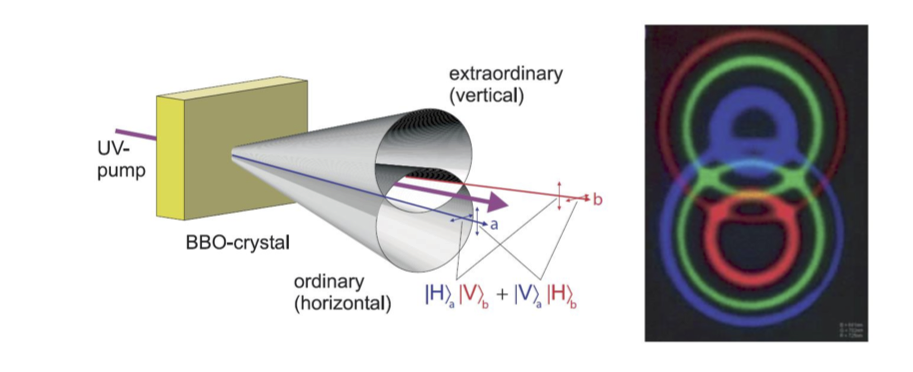
\includegraphics[scale=0.7]{./figures/cones.png}
 \caption{Cones created after the BBO \cite{physikwiki}[p. 9]}
 \label{fig:cones}
\end{figure}

\subsubsection{BBO}
\subsubsection{Waveplates}
\subsubsection{Prismas}
\subsubsection{Stages, Fibers and Detectors}

%%%%%%%%%%%%%%%%%%%%%%%%%%%%%%%%%%%%%%%%%%%%%%%%
%%%%%%%%%%%%%%%%%%%%%%%%%%%%%%%%%%%%%%%%%%%%%%%%
\section{Results}
The full document and the results contained in a QTI file and a Excel sheet can be found under \cite{github}
\subsection{Visibility}
requirement: $vis > \frac{1}{\sqrt{2}} = 0.707$\\

\noindent \textbf{H/V - Basis:}\\

$V_{HV}= (0.918 \pm 0.047) > \frac{1}{\sqrt{2}}$\\
\\
\textbf{X$^+$/X$^-$ - Basis before optimization}\\

$V_{X^+ X^- before}=(0.650 \pm 0.087) < \frac{1}{\sqrt{2}}$\\
\\
\textbf{X$^+$/X$^-$ - Basis}\\

$V_{X^+ X^- }=(0.843 \pm 0.032) > \frac{1}{\sqrt{2}}$\\

\subsection{Bell-Measurements}
$E(\alpha, \beta) = (-0.611 \pm 0.036)$\\
$E(\alpha, \beta ') = (0.765 \pm 0.041)$\\
$E(\alpha, \beta) = (-0.715\pm 0.038)$\\
$E(\alpha, \beta) = (-0.500 \pm 0.032)$\\

$$S(\alpha, \alpha ', \beta , \beta ') = (-2.591 \pm 0.074)$$

$$|S| > 2$$\\

\noindent For every single measurement, an \textbf{uncertainty of 5$\%$} was assumed.\\
The uncertainties of the results are calculated with Gaussian error propagation.




%%%%%%%%%%%%%%%%%%%%%%%%%%%%%%%%%%%%%%%%%%%%%%%%
%%%%%%%%%%%%%%%%%%%%%%%%%%%%%%%%%%%%%%%%%%%%%%%%
\section{Discussion}
Since we never came as far as to do actual measurements, the discussion will be divided into 2 parts:

\subsection{Execution of the Experiment}
The first 3 days were spent practicing alignment, learning how to use the equipment and some of the tricks, experimentalists use, so an analysis of possible error sources, improvements as well as things that worked well, is difficult.\\
From the speed, we picked up on the last day, where it was finally possible to do a reliable pre-alignment and couple the beams into the detector in a reasonable time, one can conclude, that the setup and equipment shouldn't prevent one from executing the experiment.\\
One possible error that showed up, though, was a mismatch of quality between the 2 detectors. Swapping the signals showed a difference of about a factor of 2. This could be easily accounted for at the stage of the experiment, where we had to end, though.\\
Especially in a training environment, one has to take into account unclean of faulty optical elements.\\
Without having finished the experiment and due to our general inexperience in the workings of optics experiments, it is not possible to exactly pinpoint any experimental or equipment errors.

\subsection{Bell-Violation}
From the data, that was provided, it is possible to violate the CHSH inequality.\\
For the visibility measurement, the mean was taken of all 4 combinations in each basis, while the uncertainty stems from standard deviation and student-t correction.\\
The H/V-visibility is clearly greater than $1/\sqrt{2}$ as is the X+/X- visibility after optimizing Bob's BBO.\\
The X+/X- measurements before though, clearly not suffice the requirement und thus where discarded.\\
\\
For the uncertainties of the expectation values $E(\alpha, \beta)$, an error of 5\% was assumed for every single measurement. This seems to be more than enough, since the measurement itself is already an average.\\
Gaussian error-propagation was assumed for the calculation, leading up to the result for S.\\
\\
Since the result clearly violates the inequality, one can conclude, that also a to small assumed error, wouldn't change the outcome (10\% uncertainties lead to a mere $(-2.59 \pm 0.15)$ result and thus still violating the inequality easily).


%%%%%%%%%%%%%%%%%%%%%%%%%%%%%%%%%%%%%%%%%%%%%%%%
%%%%%%%%%%%%%%%%%%%%%%%%%%%%%%%%%%%%%%%%%%%%%%%%

\bibliography{protocol.bib}
\bibliographystyle{plain}

\end{multicols}
\end{document}